\documentclass{article}
\usepackage[utf8]{inputenc}
\usepackage{graphicx}
\usepackage{float}

\title{Project ShareCar - Requirements Engineering}

\author{Isaac Paulo Betuel Mabiala\\ (pg41074@alunos.uminho.pt) \and Rapahel Pinheiro \\ (pg37160@alunos.uminho.pt) \and José André Martins Pereira\\ (a82880@alunos.uminho.pt) \and Ricardo André Gomes Petronilho\\ (a81744@alunos.uminho.pt)}

\date{January 2020}

\begin{document}

\maketitle

\section{Contextualization}

\hspace{5mm} More often we see an increase of numbers of vehicles driving on city streets - especially large cities. This high number of cars generates many problems, both for society and for the environment.

\hspace{5mm} The time spent by people on their daily commute has been increasing, which greatly diminishes their life quality. In addition, issues such as noise and air pollution endangers the health of people and the planet as a whole.

\hspace{5mm} Thus, our company X analyzed one of the major promoters of this problem: the non-intelligent use of automobile resources.

\hspace{5mm} This misuse refers to the fact that most cars on the road contain many seats, but only used by a few or a single person. According to a study in the United States, people spend 75 \% of their time driving their car alone.

\subsection{Project objectives}
\hspace{5mm} Therefore, the solution to this problem was the creation of an application that brings together people who have the same trips, at the same time, so they can share a car, share expenses and at the mean time contribute for the environment.

\hspace{5mm} So here is an example: Maria has a five-seat car, signs up to the application and offers a trip that will take place on December 19, 2019, from Braga to Lisbon, at 9:00 am and returns at 08:00 pm on the same day. João and Rita, from Braga, intend to go to Lisbon at the same times as Maria. As they are all registered, the application will bring them together for car sharing and of course sharing travel expenses.

\hspace{5mm} The positive point of this example are that the misuse of three vehicles (Maria, João and Rita) has been avoided, the traveling prices for each has been reduced, and it has contributed for the reduction of pollution to the environment and the amount of cars driving on the roads. Considering this example on a large scale, that is to say thousands of users, will gradually make better use of car resources and thus reduce environmentally harmful emissions.

\hspace{5mm} The following graphs are the responses to a survey conducted at the University of Minho for students.

\begin{figure}[H]
    \centering
	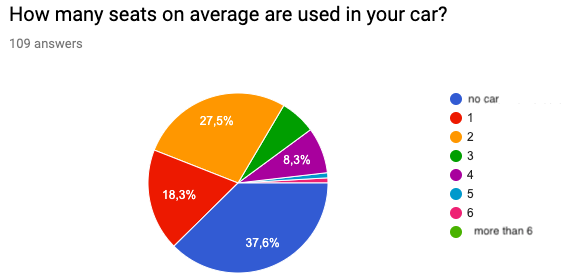
\includegraphics[scale=0.50]{g2.png}
	\caption{Survey conducted to the students of the University of Minho.}
	\label{img:duc2}
\end{figure}

\section{The solution}

\hspace{5mm}The ideal solution to solve this problem is to develop an application, which the main objective is to get people together, that want to go on the same trip by sharing the same vehicle.

\hspace{5mm} Trips are created by users, which can be viewed by others. Thus other users can join trips or be recommended by the application itself.

\section{Functionalities of Application}

\begin{itemize}
    \item Register account
    \item Create trip
    \item Get on a trip
    \item Get out a trip
    \item Give rating
    \item Search a trip
    \item etc.
\end{itemize}{}

\end{document}
